\documentclass[12pt,oneside]{report}
\usepackage[a4paper,left=4.2cm,right=2.5cm,top=2.85cm,bottom=2.85cm,headheight=16pt,headsep=18pt,footskip=30pt]{geometry}
\usepackage{fontspec}\setmainfont[Path=./,UprightFont=TIMES.TTF,BoldFont=TIMESBD.TTF,ItalicFont=TIMESI.TTF,BoldItalicFont=TIMESBI.TTF]{Times New Roman}
\usepackage{graphicx,setspace,titlesec,tocloft,array,booktabs,longtable,enumitem,amsmath,caption,xcolor,listings,float,tikz,atbegshi,eso-pic,ragged2e,placeins,fancyhdr,draftwatermark}
\usetikzlibrary{positioning,arrows.meta,shapes.geometric,calc,fit,backgrounds}
\usepackage[hidelinks]{hyperref}
\onehalfspacing\setlength{\emergencystretch}{3em}\captionsetup{font=small,labelfont=bf,skip=6pt}
\let\oldunderscore\_\renewcommand{\_}{\oldunderscore\allowbreak}
\renewcommand{\topfraction}{0.9}\renewcommand{\bottomfraction}{0.8}\renewcommand{\textfraction}{0.07}\renewcommand{\floatpagefraction}{0.75}
\titleformat{\chapter}[display]{\normalfont\LARGE\bfseries\centering}{Chapter \thechapter}{1ex}{\MakeUppercase}\titlespacing*{\chapter}{0pt}{-10pt}{20pt}
\titleformat{\section}{\normalfont\fontsize{14}{17}\bfseries}{\thesection}{0.6em}{}\titlespacing*{\section}{0pt}{18pt}{10pt}
\titleformat{\subsection}{\normalfont\fontsize{12}{15}\bfseries}{\thesubsection}{0.6em}{}\titlespacing*{\subsection}{0pt}{10pt}{6pt}
\newcommand{\ProjTitle}{Real-Time AI Governance Audit Pipeline}
\pagestyle{fancy}\fancyhf{}\fancyhead[L]{\textit{\ProjTitle}}\fancyhead[R]{2026--2027}\fancyfoot[L]{Department of AIML}\fancyfoot[R]{\thepage}\fancyheadoffset[L]{0.69cm}\fancyheadoffset[R]{0.70cm}\fancyfootoffset[L]{0.69cm}\fancyfootoffset[R]{0.70cm}\renewcommand{\headrulewidth}{0pt}\renewcommand{\footrulewidth}{0pt}
\fancypagestyle{plain}{\fancyhf{}\fancyhead[L]{\textit{\ProjTitle}}\fancyhead[R]{2026--2027}\fancyfoot[L]{Department of AIML}\fancyfoot[R]{\thepage}\renewcommand{\headrulewidth}{0pt}\renewcommand{\footrulewidth}{0pt}}
\fancypagestyle{front}{\fancyhf{}\fancyfoot[R]{\thepage}\renewcommand{\headrulewidth}{0pt}\renewcommand{\footrulewidth}{0pt}}
\AddToShipoutPictureFG{\begin{tikzpicture}[overlay,remember picture]\draw[line width=1pt]([shift={(3.51cm,-2.24cm)}]current page.north west) rectangle ([shift={(-1.8cm,2.24cm)}]current page.south east);\end{tikzpicture}}
\SetWatermarkText{
\includegraphics[width=8cm]{logo.png}}\SetWatermarkScale{1}\SetWatermarkAngle{0}\SetWatermarkColor[gray]{0.9}\SetWatermarkHorCenter{11.355cm}\SetWatermarkVerCenter{14.85cm}
\definecolor{codebg}{rgb}{0.96,0.96,0.98}\lstdefinestyle{code}{backgroundcolor=\color{codebg},basicstyle=\ttfamily\scriptsize,breaklines=true,frame=single,columns=fullflexible,keepspaces=true}\lstset{style=code}
\begin{document}
\pagenumbering{roman}
\setcounter{page}{1}
\pagestyle{fancy}
\begin{titlepage}
\thispagestyle{empty}

\begin{center}
{\Large\textbf{RV COLLEGE OF ENGINEERING\textsuperscript{\textregistered}}}\\[0.15cm]
{\large\textbf{BENGALURU--560059}}\\[0.2cm]
{\normalsize (Autonomous Institution Affiliated to VTU, Belagavi)}\\[0.7cm]

{\large\textbf{DEPARTMENT OF ARTIFICIAL INTELLIGENCE AND MACHINE LEARNING}}\\[0.5cm]


\includegraphics[width=3.0cm]{rvlogo.png}\\[0.6cm]

{\fontsize{17}{21}\selectfont\textbf{Real-Time AI Governance}}\\[0.15cm]
{\fontsize{17}{21}\selectfont\textbf{Audit Pipeline}}\\[0.6cm]

{\normalsize\textit{Project Based Learning Report}}\\[0.5cm]
{\normalsize\textbf{Submitted by}}\\[0.4cm]

{\fontsize{14}{18}\selectfont
\begin{tabular}{ll}
\textbf{Aditya Ranjan} & \textbf{1RV23AI008} \\[2pt]
\textbf{Arindam Gupta} & \textbf{1RV23AI021} \\[2pt]
\textbf{Gnanendra Naidu N} & \textbf{1RV23AI035}
\end{tabular}}\\[0.7cm]

{\small Project repository analysis and implementation report}\\[0.2cm]
{\normalsize\textbf{Real-Time AI Governance Audit Pipeline}}\\[0.6cm]

{\normalsize\textbf{Academic Year}}\\[0.1cm]
{\normalsize\textbf{2026 -- 2027}}
\end{center}

\end{titlepage}
\newpage
\cleardoublepage
\pagestyle{empty}
\thispagestyle{empty}

\begin{center}
{\Large\textbf{RV COLLEGE OF ENGINEERING\textsuperscript{\textregistered}}}\\[0.25cm]
{\small (Autonomous Institution Affiliated to Visvesvaraya Technological University, Belagavi)}\\[0.7cm]
{\Large\textbf{DEPARTMENT OF ARTIFICIAL INTELLIGENCE}}\\[0.15cm]
{\Large\textbf{AND MACHINE LEARNING}}\\[0.25cm]
{\small Bengaluru -- 560059}\\[1cm]

\includegraphics[width=3.0cm]{rvlogo.png}\\[0.9cm]
{\Large\underline{\textbf{CERTIFICATE}}}\\[0.6cm]
\end{center}

\begin{center}
\begin{minipage}{1.0\textwidth}
\justifying
\noindent
Certified that the project work titled \textbf{`Real-Time AI Governance Audit Pipeline'} is carried out by
\textbf{Aditya Ranjan (1RV23AI008)}, \textbf{Arindam Gupta (1RV23AI021)}, and
\textbf{Gnanendra Naidu N (1RV23AI035)}, who are bonafide students of RV College of Engineering,
Bengaluru, in partial fulfillment of the curriculum requirement of 7\textsuperscript{th} Semester
\textbf{Stream Processing and Analytics} Experiential Learning during the
academic year \textbf{2026--2027}. It is certified that all corrections/suggestions indicated for
the Internal Assessment have been incorporated in the report. The report has been approved as it
satisfies the academic requirements in respect of experiential learning work prescribed
by the institution.
\end{minipage}
\end{center}

\vspace{1.5cm}
\begin{center}
\begin{tabular*}{\textwidth}{@{\extracolsep{\fill}}cc}
\begin{tabular}[t]{c}
\textbf{Signature of Faculty In-charge}\\
\textbf{Dept. of AIML, RVCE}
\end{tabular}
&
\begin{tabular}[t]{c}
\textbf{HoD}\\
\textbf{Dept. of AIML, RVCE}
\end{tabular}
\end{tabular*}

\vspace{1cm}
\noindent
\textbf{\underline{External Examination}}

\begin{tabular*}{\textwidth}{@{\extracolsep{\fill}}ll}
\textbf{Name of Examiners} &
\textbf{Signature with date} \\
\textbf{1} & \\[0.25cm]
\textbf{2} &
\end{tabular*}
\end{center}
\vfill

\thispagestyle{empty}

\pagestyle{fancy}\tableofcontents\thispagestyle{fancy}\clearpage\pagenumbering{arabic}\pagestyle{fancy}

\chapter{Introduction}
\section{Objective}
This report analyses the Git repository \textit{AI-Governance-Audit-Pipeline}, a runnable reference implementation for collecting AI-governance evidence, detecting compliance conditions, scoring risk, persisting findings, and supporting evidence-grounded investigation and review. It follows the supplied SPA report format: formal chapters, numbered sections, source references, and an evidence appendix.
\section{Scope}
The analysis covers the source tree, schemas, rule catalogue, Kafka Streams processor, Python services, database schema, deployment files, evaluation material, and the dated evidence package. It does not claim that framework mappings establish legal conformity; the repository itself correctly treats them as evidence-routing decisions.
\section{Executive summary}
The system is a modular event-to-framework pipeline. Five independent adapters normalize source events into a canonical contract and publish to dedicated topics. A stateful Kafka Streams processor evaluates 16 rules, then a risk scorer and idempotent PostgreSQL sink complete the path. Tableau views expose operational and compliance reporting. Optional Amazon Bedrock Investigator and Evidence Reviewer agents add bounded, durable, advisory analysis. The governance framing follows contemporary risk-management guidance from NIST, ISO, the OECD, UNESCO, and the EU AI Act \cite{nist2023,nistgenai2024,iso42001,oecd2024,unesco2021,euaiact2024}.

\chapter{Problem Definition and Objectives}
\section{Problem statement}
AI systems generate evidence across identity, infrastructure, pipelines, model registries, and LLM gateways. Without a shared event contract and durable correlation, governance teams cannot reliably connect raw activity to controls, risk, evidence, and review outcomes. The project addresses this by combining source-specific adapters, event-time rules, risk scoring, persistence, and human-review boundaries. This emphasis on traceability and lifecycle controls is consistent with recent AI governance guidance \cite{nist2023,iso42001,euaiact2024,owasllm2025}.
\section{Objectives}
\begin{enumerate}[leftmargin=*]\item Normalize five heterogeneous producer systems into one versioned governance event.\item Detect 16 executable governance controls with windows and stateful joins.\item Preserve event, finding, score, evidence, and review identity end to end.\item Provide deterministic and machine-learning risk signals without replacing the deterministic baseline.\item Demonstrate recovery, testing, traceability, and advisory agent review.\end{enumerate}

\chapter{Literature Review}
\section{Recent governance and engineering literature}
Recent guidance treats AI governance as a lifecycle practice involving accountability, documentation, measurement, monitoring, and human oversight rather than a one-time model check \cite{nist2023,nistgenai2024,iso42001,oecd2024,unesco2021,euaiact2024,stanford2024}. Security guidance also highlights prompt injection, data leakage, excessive agency, and supply-chain risks in LLM-enabled systems \cite{owasllm2025,mitreatlas2024,google2023}. The project responds to these themes through immutable evidence, explicit contracts, bounded agent loops, separate service identities, and a human-review terminal state.
\begin{table}[H]\centering\small\begin{tabular}{|p{2.8cm}|p{1.0cm}|p{4.1cm}|p{4.0cm}|}\hline
\textbf{Source} & \textbf{Year} & \textbf{Main contribution} & \textbf{Design implication for this project}\\\hline
NIST AI RMF \cite{nist2023} & 2023 & Govern, map, measure, and manage AI risk & Rule catalogue, evidence, scores, and review states\\\hline
NIST GenAI Profile \cite{nistgenai2024} & 2024 & GenAI-specific risk actions and lifecycle profile & Bedrock agent boundaries and evidence grounding\\\hline
ISO/IEC 42001 \cite{iso42001} & 2023 & AI management-system requirements and continual improvement & Durable controls, ownership, audit history\\\hline
EU AI Act \cite{euaiact2024} & 2024 & Risk-tiered obligations, transparency, and governance & Framework labels and human escalation\\\hline
OWASP LLM Top 10 \cite{owasllm2025} & 2025 & Common LLM application security risks & Prompt isolation, structured tools, bounded execution\\\hline
Kafka Streams documentation \cite{kafkastreams2024} & 2024 & Event-time state, joins, and processing guarantees & Windowed failed-login detection and promotion joins\\\hline
Kubernetes documentation \cite{kubernetes2024} & 2024 & Probes, scaling, disruption budgets, and workload operation & Resilient service deployment and recovery checks\\\hline
RAG survey literature \cite{ragsurvey2024} & 2024 & Retrieval grounding and evaluation concerns & Evidence snapshots and citation validation\\\hline
\end{tabular}\caption{Comparison of recent sources and the corresponding implementation decision.}\end{table}
\section{Research gap and project position}
The literature provides principles, controls, and security taxonomies, but governance teams still need an operational evidence path that connects source activity to a finding, score, stored record, and review outcome. This repository occupies that implementation gap. Its contribution is systems integration and measurable traceability, not a new foundation model or a claim of legal certification.

\chapter{System Architecture}
\section{High-level architecture}
\begin{figure}[H]
\centering
\resizebox{0.98\textwidth}{!}{%
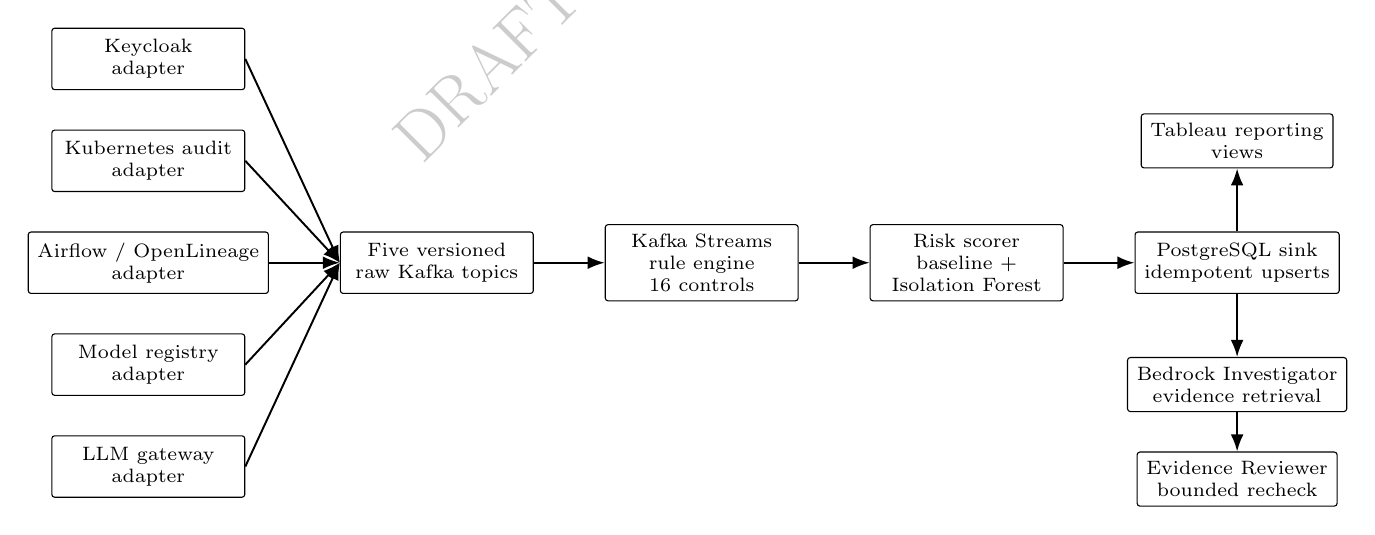
\begin{tikzpicture}[block/.style={draw,rectangle,rounded corners=1pt,align=center,minimum height=0.78cm,minimum width=2.45cm,font=\scriptsize},smallblock/.style={draw,rectangle,rounded corners=1pt,align=center,minimum height=0.62cm,minimum width=2.15cm,font=\scriptsize},line/.style={-Latex,line width=0.7pt},node distance=0.5cm and 0.55cm]
\node[block] (identity) {Keycloak\\adapter};
\node[block,below=of identity] (kube) {Kubernetes audit\\adapter};
\node[block,below=of kube] (airflow) {Airflow / OpenLineage\\adapter};
\node[block,below=of airflow] (registry) {Model registry\\adapter};
\node[block,below=of registry] (llm) {LLM gateway\\adapter};
\node[block,right=0.9cm of airflow] (topics) {Five versioned\\raw Kafka topics};
\node[block,right=0.9cm of topics] (engine) {Kafka Streams\\rule engine\\16 controls};
\node[block,right=0.9cm of engine] (risk) {Risk scorer\\baseline +\\Isolation Forest};
\node[block,right=0.9cm of risk] (sink) {PostgreSQL sink\\idempotent upserts};
\node[smallblock,above=0.8cm of sink] (tableau) {Tableau reporting\\views};
\node[smallblock,below=0.8cm of sink] (investigator) {Bedrock Investigator\\evidence retrieval};
\node[smallblock,below=of investigator] (reviewer) {Evidence Reviewer\\bounded recheck};
\foreach \source in {identity,kube,airflow,registry,llm} {\draw[line] (\source.east) -- (topics.west);}
\draw[line] (topics) -- (engine);\draw[line] (engine) -- (risk);\draw[line] (risk) -- (sink);
\draw[line] (sink.north) -- (tableau.south);\draw[line] (sink.south) -- (investigator.north);\draw[line] (investigator) -- (reviewer);
\end{tikzpicture}
}%
\caption{High-level architecture derived from the repository services, deployment manifests, and documented event flow.}
\end{figure}
The architecture separates producers, stream processing, scoring, storage, and reporting. Local Compose uses Redpanda and PostgreSQL; AWS deployment definitions provide MSK, EKS, RDS, ECR, IAM, VPC, and security groups. Kafka topics and JSON contracts are the primary integration boundary. The design follows documented event-stream processing and cloud-native operational patterns \cite{kafkastreams2024,redpanda2024,kubernetes2024,terraform2024}.
\section{Module responsibilities}
\begin{longtable}{p{0.27\textwidth}p{0.63\textwidth}}\toprule Component & Responsibility\\\midrule
Producer adapters & Five standalone HTTP services for Keycloak, Kubernetes audit, Airflow/OpenLineage, model registry, and LLM gateway.\\
Stream processor & Java Kafka Streams topology with event-time windows, joins, rule catalog, and finding creation.\\
Risk scorer & Online Isolation Forest comparison with a deterministic severity-frequency baseline.\\
PostgreSQL sink & Idempotent event and finding upserts plus indexed evidence and reporting views.\\
Agents & Bedrock Investigator and Evidence Reviewer with durable jobs, structured contracts, and bounded revision.\\
Deployment & Docker Compose, Kubernetes manifests, Terraform infrastructure, and Tableau setup.\\\bottomrule\end{longtable}
\section{Data flow}
\begin{lstlisting}
source -> adapter -> raw topic -> canonical event -> rule engine
       -> finding -> risk scorer -> PostgreSQL -> Tableau / agents
\end{lstlisting}

\chapter{Data Sources and Contracts}
\section{Producer groups}
Each producer has its own adapter, health/readiness/metrics endpoints, image, deployment, scaling policy, IAM role, and topic. This reduces coupling and permits source-specific validation while maintaining a common downstream contract.
\section{Canonical event contract}
The versioned governance-event schema captures identity, source, timestamps, actor, object, action, attributes, and evidence metadata. Mappers remove source-specific variation while preserving useful provenance. Safe dead-letter handling prevents malformed input from silently entering the main path. This is aligned with current software supply-chain and observability practice \cite{openssf2024,opentelemetry2024}.
\section{Topics and integration}
The repository defines one raw topic per producer and separate consumer groups for rule processing, scoring, persistence, and evaluation. Six partitions and independent consumer groups support parallelism; offsets, keys, and event IDs enable reconciliation.
\begin{figure}[H]\centering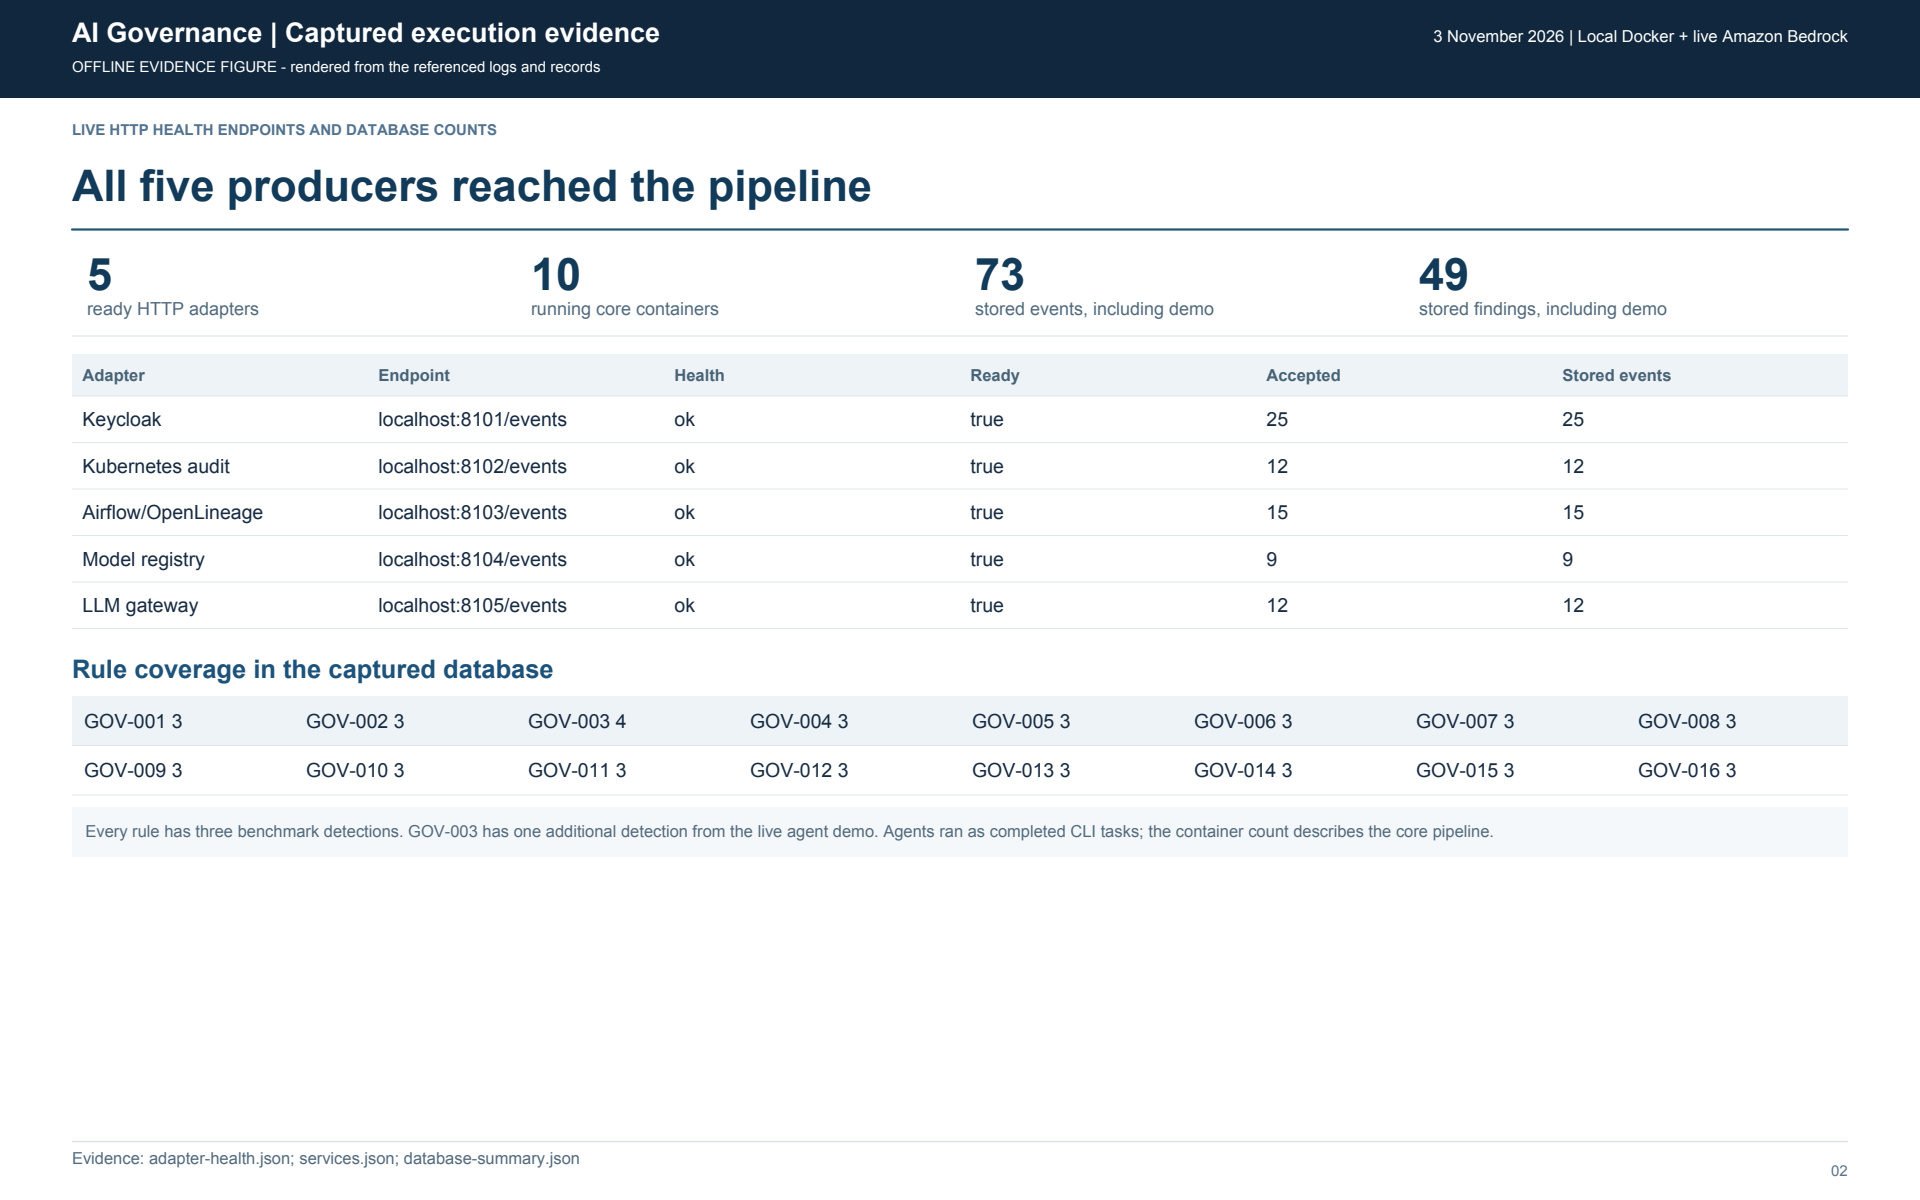
\includegraphics[width=0.86\textwidth]{figures/02-producer-health.png}\caption{Captured health and accepted-event evidence for the five producer adapters.}\end{figure}

\chapter{Rule Engine and Framework Mapping}
\section{Executable controls}
The 16-rule catalogue in \texttt{config/rules.yml} maps each control to NIST AI RMF 1.0, ISO/IEC 42001:2023, EU AI Act, NIST SP 800-53 Rev. 5, and GDPR. The Java implementation contains stateless predicates, a five-minute failed-login window with one-minute grace, and stateful promotion joins. The separation between a control mapping and a legal conclusion follows the risk-management approach in \cite{nist2023,iso42001,euaiact2024}.
\section{Finding record}
Findings retain rule ID, severity, triggering event identity, timestamps, framework labels, evidence, and processing metadata. This makes a control result inspectable rather than a transient alert.
\begin{figure}[H]\centering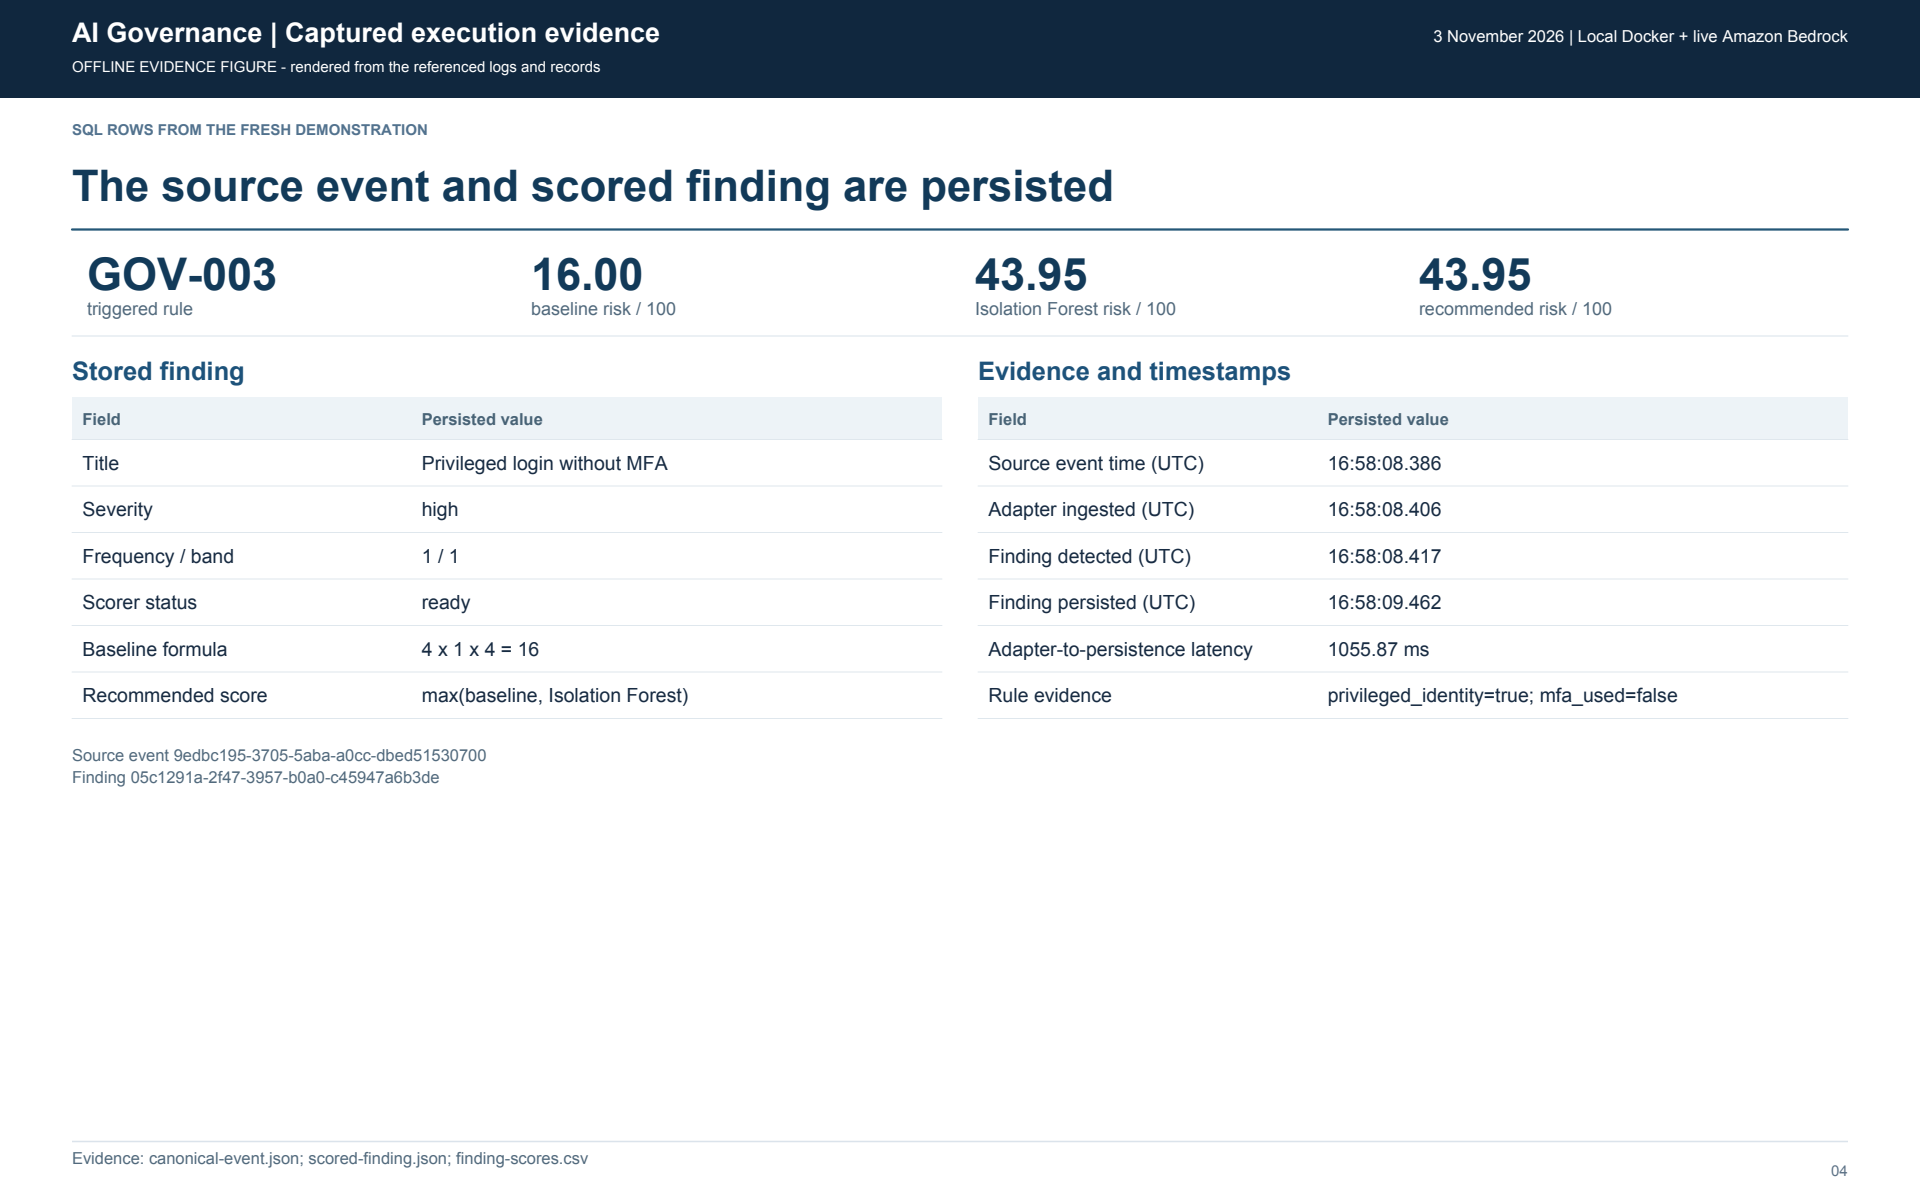
\includegraphics[width=0.92\textwidth]{figures/04-persisted-finding.png}\caption{Persisted finding evidence showing the triggering event, rule, scores, and timestamps.}\end{figure}

\chapter{Risk Scoring, Storage and Reporting}
\section{Risk scoring}
The deterministic baseline combines a 1--5 frequency bucket with severity and produces a normalized 0--100 score. An online Isolation Forest maintains bounded history and stores its score, delta, readiness status, and recommended score beside the baseline. The ML signal is comparative and does not remove the explainability of the rule result. The implementation uses the established scikit-learn API and keeps the baseline visible for auditability \cite{scikitlearn2024}.
\section{Persistence model}
PostgreSQL stores raw events, findings, evidence, risk scores, jobs, agent reports, reviews, and audit history. Upserts and indexes support idempotency and case retrieval. Tableau views cover framework status, risk trend, incident history, and pipeline latency.
\section{Agent integration}
The Investigator retrieves eligible evidence and writes a structured report. The Evidence Reviewer checks citations and completeness, can request at most one revision, and may terminate in human review. Reports and evidence snapshots remain immutable; agents do not remediate systems. This bounded pattern reflects current agent observability and responsible-agent guidance \cite{bedrock2025,cloudwatch2025,agentsurvey2024}.
\begin{figure}[H]\centering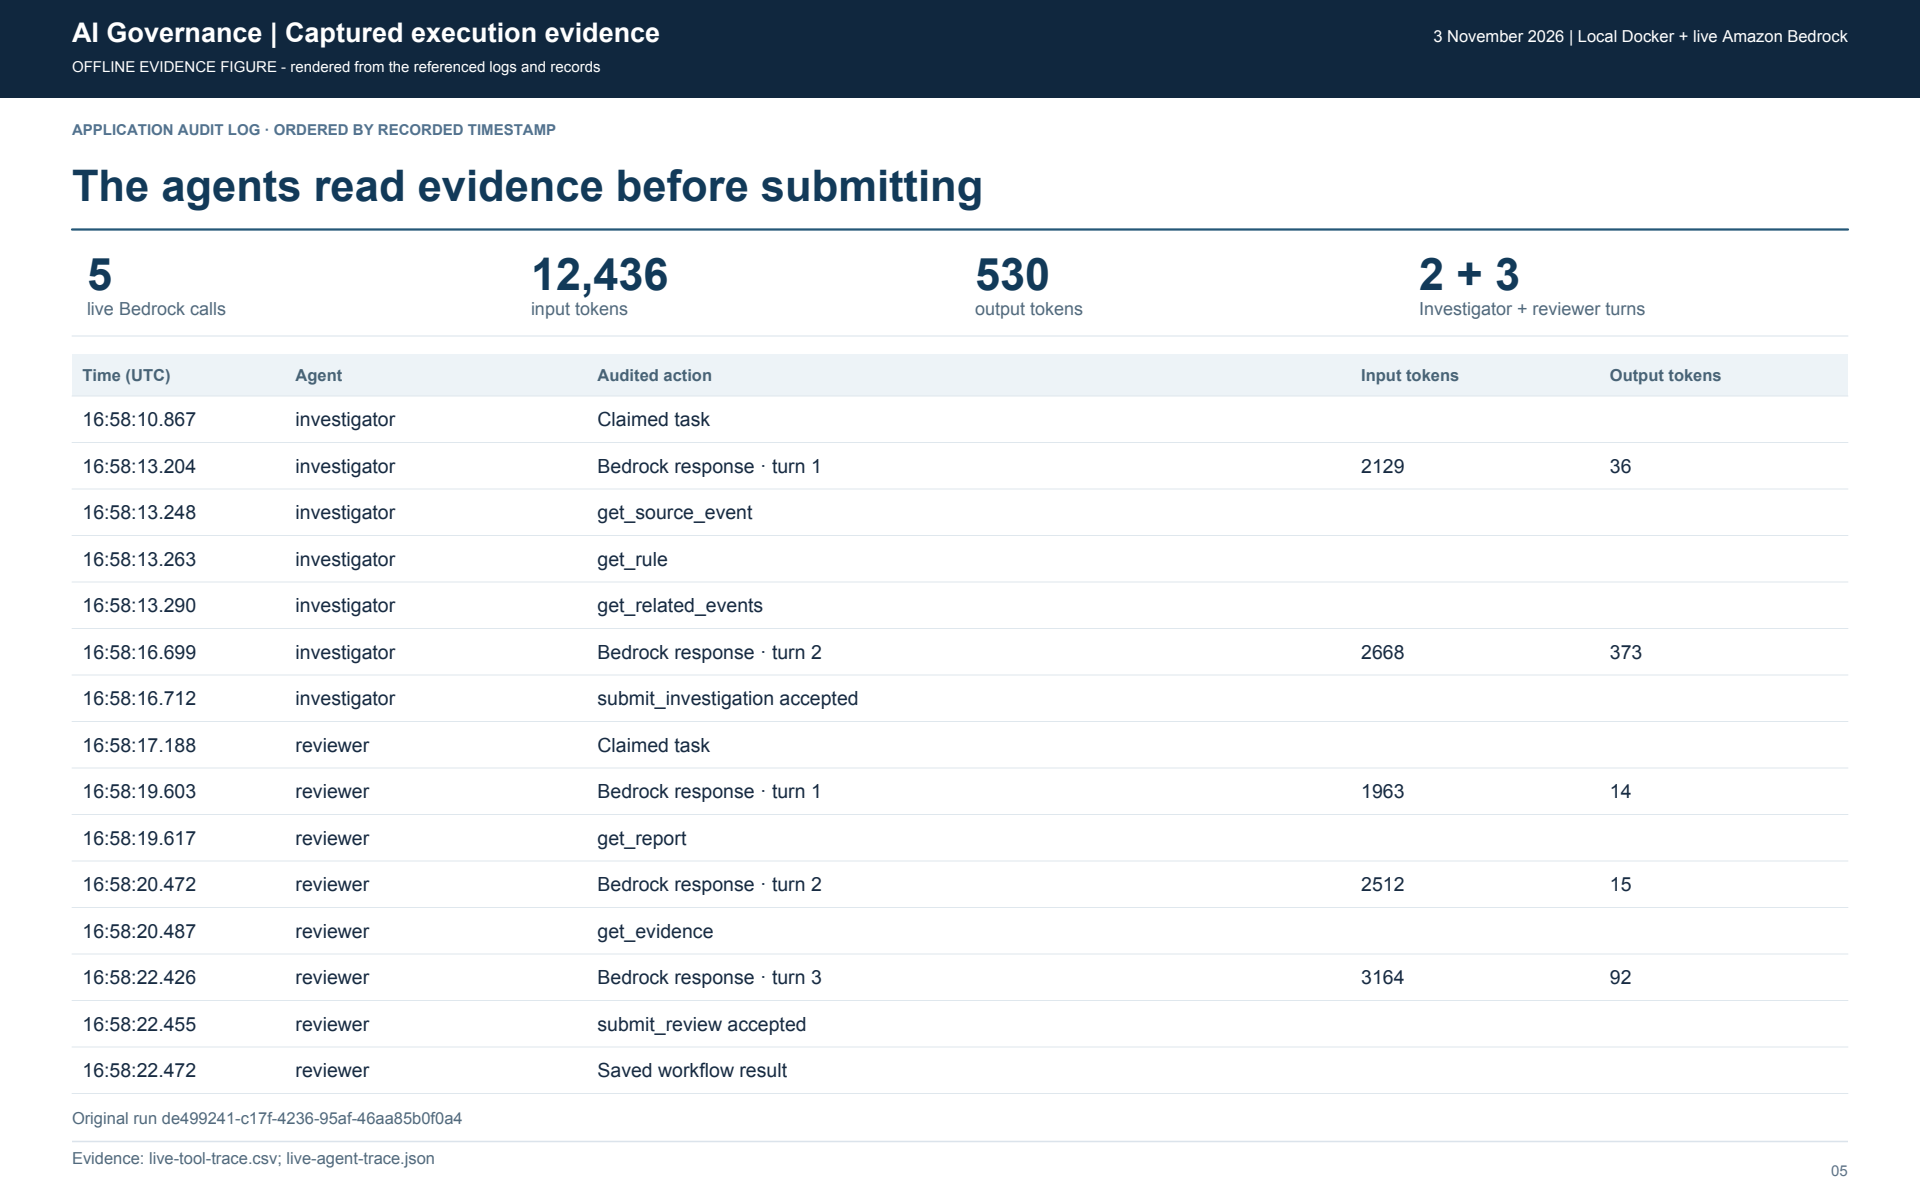
\includegraphics[width=0.90\textwidth]{figures/05-agent-tool-trace.png}\caption{Live tool trace for the Investigator and Evidence Reviewer.}\end{figure}

\chapter{Deployment and Operations}
\section{Local operation}
The documented local path uses Docker Desktop with at least 6 GB available: copy \texttt{.env.example}, start Compose, inject labelled evaluation events, and export a report. Redpanda stands in for MSK and a PostgreSQL container stands in for RDS.
\section{AWS operation}
Terraform provisions a VPC, three-broker MSK, EKS, RDS, ECR, security groups, and workload IAM. Kubernetes manifests define services, probes, HPAs, PDBs, and consumer scaling. The deployment instructions correctly require image publication, secret creation, placeholder replacement, and an evaluation before recording results.
\section{Resilience and controls}
Idempotent writes, retrying producers, replication factor three, minimum ISR two, consumer groups, and reconciliation checks address loss and restart scenarios. Operational scripts pause and resume services; failure procedures distinguish the local single-broker demonstration from AWS broker failover.

\chapter{Testing and Results}
\section{Verification coverage}
The repository includes Python, Java, mapper, integration, settings, reviewer, topology, scorer, and evaluation tests. Requirements traceability links each major requirement to implementation and verification. The 3 November evidence package records 83 agent tests passed in 9.65 seconds.
\section{Measured functional run}
\begin{table}[H]\centering\small\begin{tabular}{lrrrrr}\toprule Scenario & Events & Exp./Obs. & Precision & Recall & Throughput\\\midrule
Baseline & 72 & 48/48 & 1.0000 & 1.0000 & 130.90/s\\
Processor replacement & 72 & 48/48 & 1.0000 & 1.0000 & 11.50/s\\
Broker restart & 72 & 48/48 & 1.0000 & 1.0000 & 11.48/s\\
Independent adapters & 72 & 48/48 & 1.0000 & 1.0000 & 667.12/s\\\bottomrule\end{tabular}\caption{Repository-reported local evaluation results.}\end{table}
The fresh 3 November evidence also reports 72 synthetic source-shaped events, 48 expected findings across all 16 rules, p50 353.84 ms, p95 1,878.88 ms, p99 2,181.69 ms, and 39.04 events/s over the observed persistence interval. These are small-workload measurements, not general model-accuracy claims.
\begin{figure}[H]\centering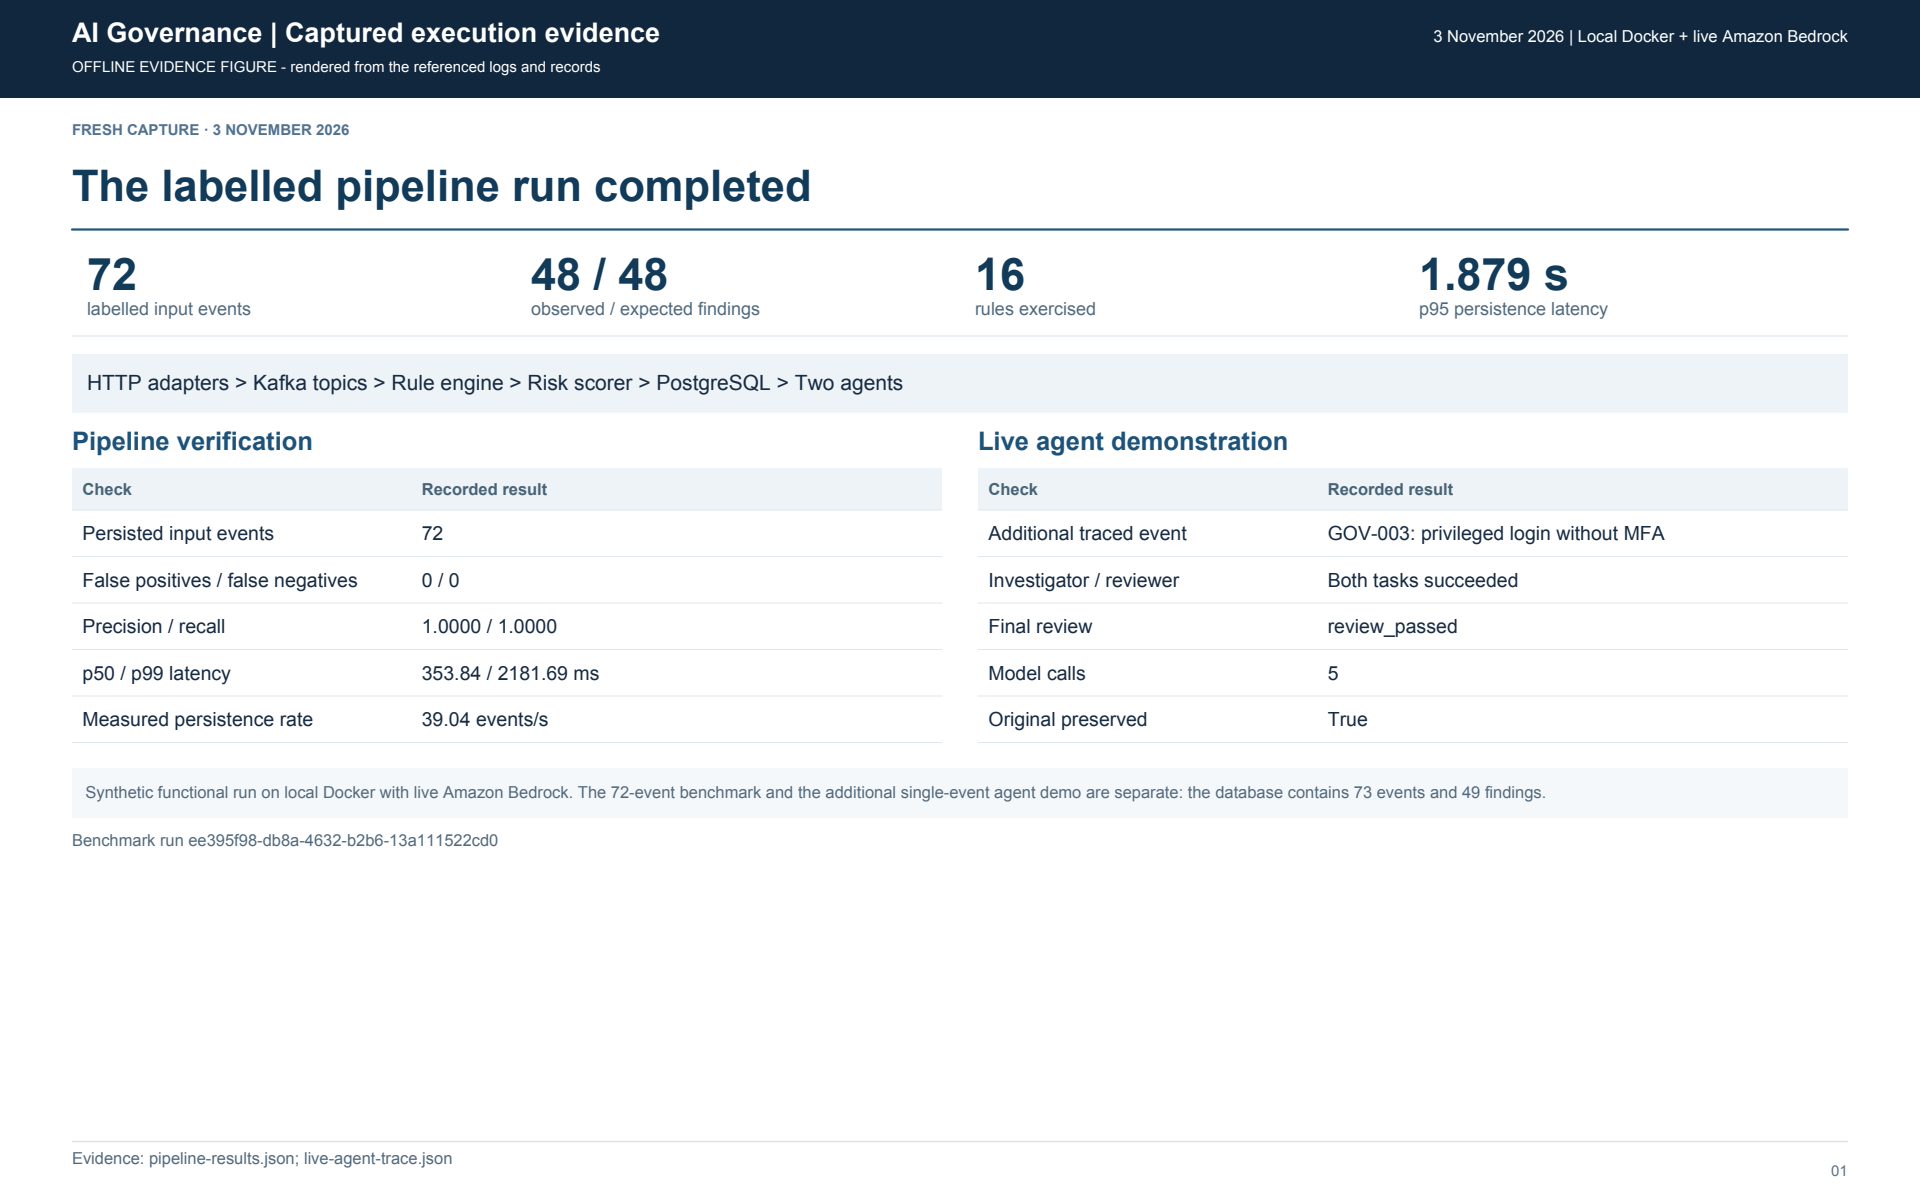
\includegraphics[width=0.92\textwidth]{figures/01-pipeline-run.png}\caption{Pipeline benchmark evidence for the labelled functional run.}\end{figure}
\begin{figure}[H]\centering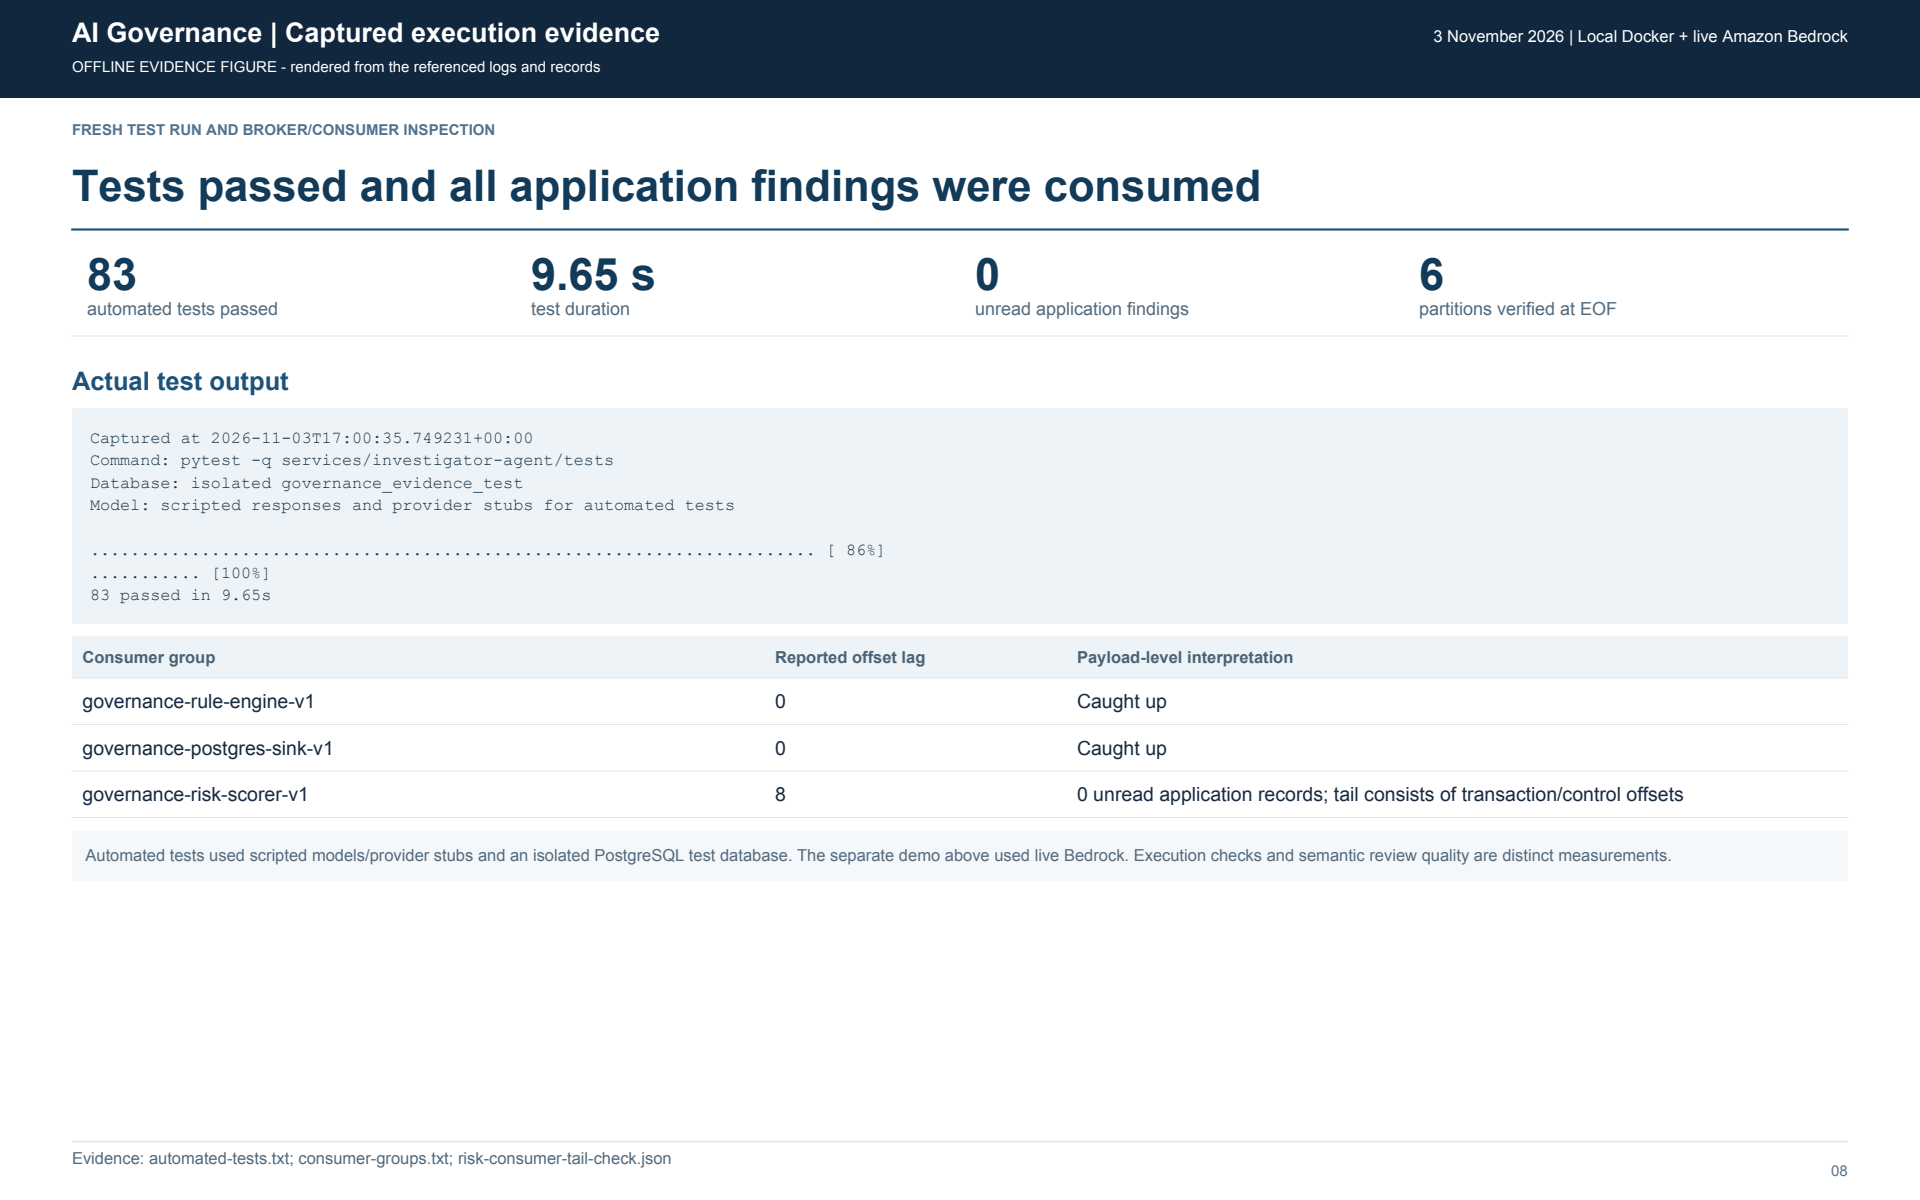
\includegraphics[width=0.92\textwidth]{figures/08-tests-and-consumer-checks.png}\caption{Automated tests and consumer-tail verification.}\end{figure}

\chapter{Agentic AI Evaluation and Limitations}
\section{Observed outcomes}
One fresh individual case completed investigation and review with \texttt{review\_passed}; the original report and evidence snapshot were preserved. A saved correction example demonstrates cited feedback, one revision, recheck, and terminal \texttt{needs\_human\_review}. CloudWatch evidence for the selected window records five Bedrock invocations, 12,436 input tokens, 530 output tokens, and 1,476.4 ms average latency.
\begin{figure}[H]\centering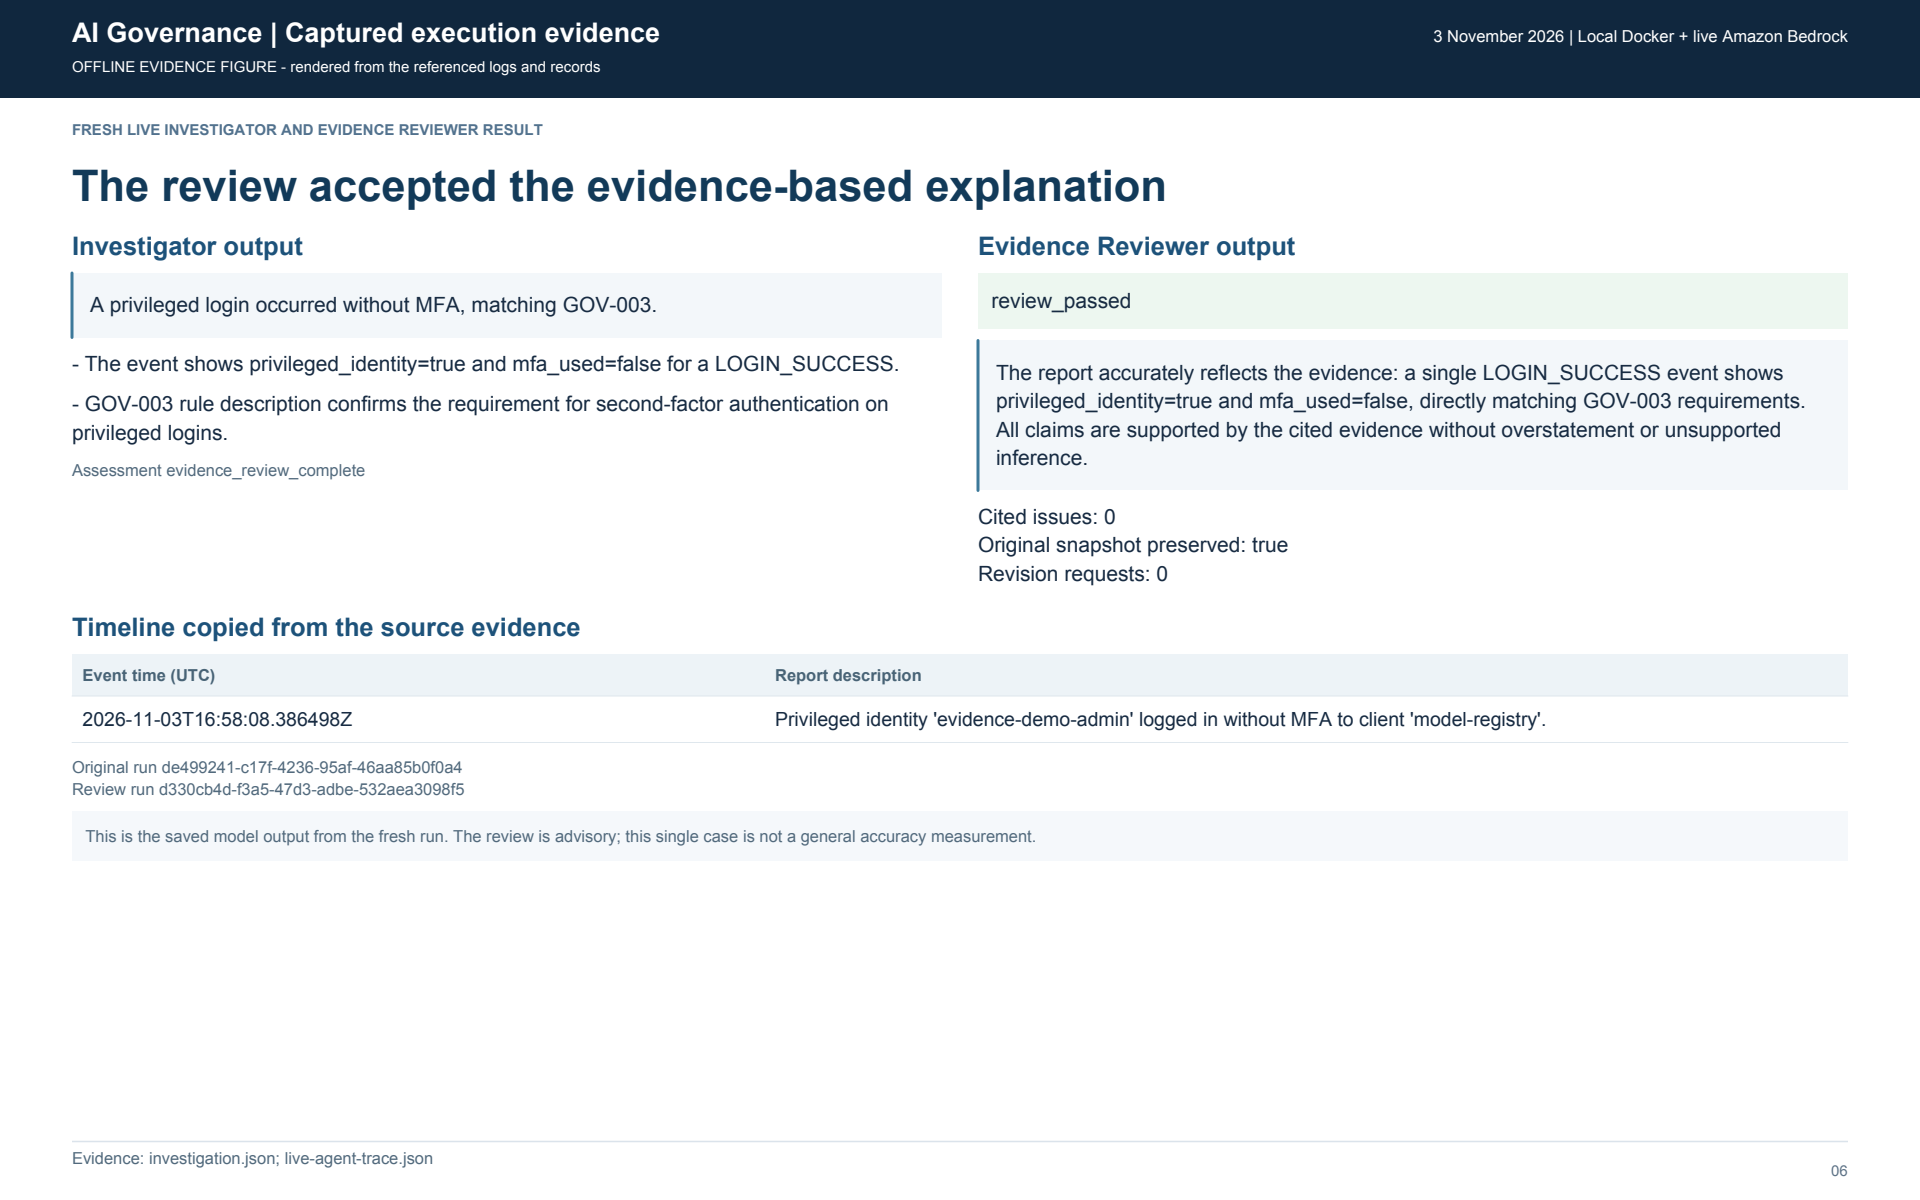
\includegraphics[width=0.92\textwidth]{figures/06-reviewed-report.png}\caption{Fresh reviewed report with preserved evidence.}\end{figure}
\begin{figure}[H]\centering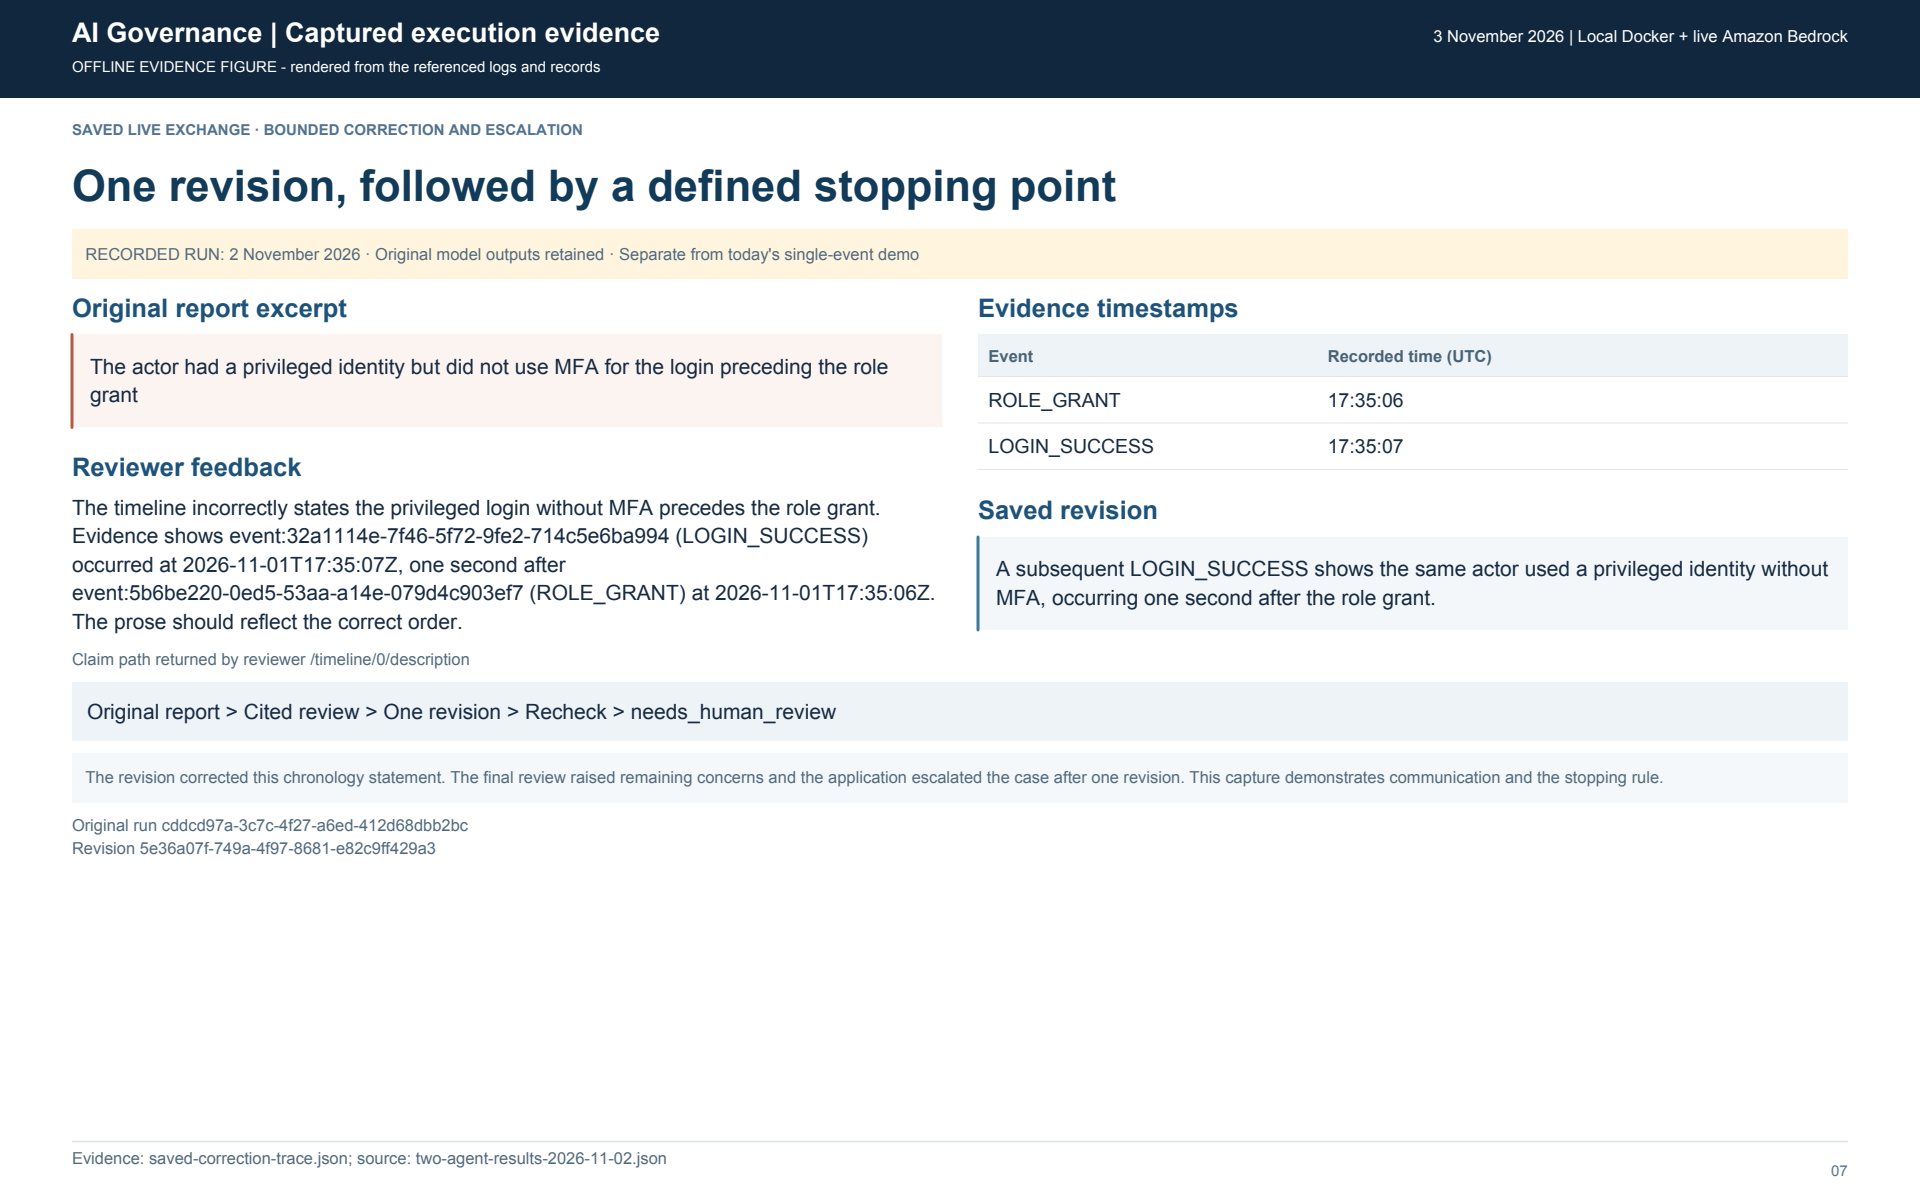
\includegraphics[width=0.92\textwidth]{figures/07-correction-and-recheck.png}\caption{Saved correction, revision, and human-escalation example.}\end{figure}
\section{Limitations}
The reviewer is advisory and must not be treated as an automatic approval gate. The evidence package contains selected demonstrations rather than corpus-wide semantic-quality evaluation. Framework labels are routing metadata, not legal conclusions. The AWS metrics are account/model/region aggregates for the selected window, while the application trace provides case-level correlation.

\chapter{Conclusion}
The project is a coherent, runnable governance-audit platform with unusually strong traceability for a reference implementation. Its strongest engineering decisions are independent adapters, explicit contracts, event-time/stateful processing, idempotent persistence, measured recovery tests, immutable evidence, and bounded agent workflows. The main adoption requirement is operational discipline: execute the documented evaluation in the target environment, retain evidence, and preserve human review for uncertain or corrected agent outcomes.

\chapter*{References}\addcontentsline{toc}{chapter}{References}
\sloppy
\begin{thebibliography}{99}
\bibitem{project} A. Ranjan, A. Gupta, and G. N. Naidu, ``AI-Governance-Audit-Pipeline,'' GitHub repository, 2026. Available: \url{https://github.com/Aditya-Ranjan1234/AI-Governance-Audit-Pipeline}
\bibitem{nist2023} E. Tabassi, ``Artificial Intelligence Risk Management Framework (AI RMF 1.0),'' NIST AI 100-1, 2023. doi:10.6028/NIST.AI.100-1.
\bibitem{nistgenai2024} NIST, ``Artificial Intelligence Risk Management Framework: Generative Artificial Intelligence Profile,'' NIST AI 600-1, 2024. Available: \url{https://doi.org/10.6028/NIST.AI.600-1}
\bibitem{iso42001} ISO/IEC, ``ISO/IEC 42001:2023 Information technology -- Artificial intelligence -- Management system,'' 2023. Available: \url{https://www.iso.org/standard/81230.html}
\bibitem{oecd2024} OECD, ``OECD AI Principles,'' updated 2024. Available: \url{https://oecd.ai/en/ai-principles}
\bibitem{unesco2021} UNESCO, ``Recommendation on the Ethics of Artificial Intelligence,'' 2021. Available: \url{https://unesdoc.unesco.org/ark:/48223/pf0000381137}
\bibitem{euaiact2024} European Parliament and Council, ``Regulation (EU) 2024/1689 (Artificial Intelligence Act),'' 2024. Available: \url{https://eur-lex.europa.eu/eli/reg/2024/1689}
\bibitem{stanford2024} Stanford Institute for Human-Centered Artificial Intelligence, ``AI Index Report 2024,'' 2024. Available: \url{https://aiindex.stanford.edu/report/}
\bibitem{owasllm2025} OWASP Foundation, ``OWASP Top 10 for Large Language Model Applications,'' 2025. Available: \url{https://owasp.org/www-project-top-10-for-large-language-model-applications/}
\bibitem{mitreatlas2024} MITRE, ``MITRE ATLAS: Adversarial Threat Landscape for Artificial-Intelligence Systems,'' 2024. Available: \url{https://atlas.mitre.org/}
\bibitem{google2023} Google, ``Secure AI Framework (SAIF),'' 2023. Available: \url{https://safety.google/cybersecurity-advancements/saif/}
\bibitem{kafkastreams2024} Apache Software Foundation, ``Kafka Streams Developer Guide,'' 2024. Available: \url{https://kafka.apache.org/documentation/streams/}
\bibitem{redpanda2024} Redpanda Data, ``Redpanda Documentation,'' 2024. Available: \url{https://docs.redpanda.com/current/}
\bibitem{kubernetes2024} Kubernetes Authors, ``Kubernetes Documentation: Workloads, Probes, Scaling and Disruptions,'' 2024. Available: \url{https://kubernetes.io/docs/}
\bibitem{terraform2024} HashiCorp, ``Terraform AWS Provider Documentation,'' 2024. Available: \url{https://registry.terraform.io/providers/hashicorp/aws/latest/docs}
\bibitem{openssf2024} OpenSSF, ``Open Source Security Foundation Scorecard Documentation,'' 2024. Available: \url{https://scorecard.dev/}
\bibitem{opentelemetry2024} OpenTelemetry Authors, ``OpenTelemetry Documentation,'' 2024. Available: \url{https://opentelemetry.io/docs/}
\bibitem{scikitlearn2024} scikit-learn Developers, ``IsolationForest API Reference,'' version 1.5, 2024. Available: \url{https://scikit-learn.org/stable/modules/generated/sklearn.ensemble.IsolationForest.html}
\bibitem{ragsurvey2024} Y. Gao et al., ``Retrieval-Augmented Generation for Large Language Models: A Survey,'' arXiv:2312.10997, revised 2024. Available: \url{https://arxiv.org/abs/2312.10997}
\bibitem{agentsurvey2024} M. Wang et al., ``A Survey on Large Language Model based Autonomous Agents,'' arXiv:2308.11432, revised 2024. Available: \url{https://arxiv.org/abs/2308.11432}
\bibitem{bedrock2025} Amazon Web Services, ``Amazon Bedrock User Guide: Agents,'' 2025. Available: \url{https://docs.aws.amazon.com/bedrock/latest/userguide/agents.html}
\bibitem{cloudwatch2025} Amazon Web Services, ``Monitor Amazon Bedrock Agents using CloudWatch Metrics,'' 2025. Available: \url{https://docs.aws.amazon.com/bedrock/latest/userguide/monitoring-agents-cw-metrics.html}
\end{thebibliography}
\end{document}
